\documentclass[12pt]{article}
\usepackage{hyperref}
\usepackage{authblk}
% Document Layout
\usepackage{natbib}
\bibliographystyle{aer}

\usepackage{geometry} % Customize document dimensions, margins, and page size.
\usepackage{fancyhdr} % Extensive control of page headers and footers.
\usepackage{titlesec} % Control over section and chapter headings.

% Font and Text
\usepackage[utf8]{inputenc} % Allows input of international characters.
\usepackage[T1]{fontenc} % Font encoding.
\usepackage[english]{babel} % Multilingual support.
\usepackage{amsmath, amsfonts, amssymb} % American Mathematical Society packages for advanced math typesetting.
\usepackage{mathptmx} % Times font
\usepackage{helvet} % Helvetica font
\usepackage{courier} % Courier font

% Graphics and Tables
\usepackage{graphicx} % Enhanced support for graphics.
\usepackage{subfigure} % or use \usepackage{subcaption} for handling sub-figures within a single figure environment.
\usepackage{float} % Improved interface for floating objects (tables, figures).
\usepackage{wrapfig} % Allows figures or tables to have text wrapped around them.
\usepackage{pgf, tikz} % Creating high-quality diagrams and figures.
\usepackage{xcolor} % Easy driver-independent access to several kinds of color tints, shades, tones, and mixes of arbitrary colors.
\usepackage{color} 
\usepackage{tabularx} % Enhanced tables.
\usepackage{booktabs} % Publication quality tables in LaTeX.

\usepackage{threeparttable}
\usepackage{longtable}
\usepackage{pdflscape}

% Set the page size and margins
\geometry{letterpaper, portrait, margin=1in}


\title{Sketch for the Conceptual Framework}
\author[1]{Zhiyao (Yao) Ma}
\affil[1]{UC Davis}
\date{\today}


\begin{document}
\maketitle
\tableofcontents
\newpage


\section{Farmers' Marketing Plan: Two-Period Dynamic Maximization Problem}

A risk-averse farmer is maximizing his expected utility on the revenue under the given harvest ($q$) over two trading periods by choosing the share of the harvest stored in the first trading period and sold later ($s$), ranging from 0 to 1. The farmer observes the first-period price first and then decides how much to store; the storage cost is captured by a discount factor. The farmer is maximizing the sum of the expected utility of two periods. This setting would give us an interior solution.

\subsection{Problem Setup}

Given:
\begin{itemize}
    \item $q$: Total harvest quantity (fixed and known)
    \item $p_1$: Price in the first trading period (observed)
    \item $p_2$: Price in the second trading period (stochastic)
    \item $s$: Share of harvest stored for the second period ($0 \leq s \leq 1$)
    \item $\delta$: Discount factor (storage cost)
    \item $U(x) = \frac{x^{1 - \gamma}}{1 - \gamma}$: the Constant Relative Risk Aversion (CRRA) utility function with $\gamma > 0, \gamma \neq 1$
    \item when $\gamma=1$, the period utility function is $ln(x)$
\end{itemize}

Revenue Equations:
\begin{align*}
    R_1 &= \left(1 - s\right) \cdot q \cdot p_1 \\
    R_2 &= s \cdot q \cdot p_2
\end{align*}

Expected Utility Function:
\begin{align}
    \max_{0 \leq s \leq 1} \left[ U(\left(1 - s\right) \cdot q \cdot p_1) + \delta \cdot E\left[U(s \cdot q \cdot p_2)\right] \right]
\end{align}

Using the CRRA utility function $U(x) = \frac{x^{1 - \gamma}}{1 - \gamma}$, the objective function becomes:
\begin{align*}
    \max_{0 \leq s \leq 1} \left[ \frac{(\left(1 - s\right) \cdot q \cdot p_1)^{1 - \gamma}}{1 - \gamma} + \delta \cdot E\left[\frac{(s \cdot q \cdot p_2)^{1 - \gamma}}{1 - \gamma}\right] \right]
\end{align*}

Factoring out constants $\frac{q^{1 - \gamma}}{1 - \gamma}$, the problem reduces to:
\begin{align}
    \max_{0 \leq s \leq 1} \left[ \left(1 - s\right)^{1 - \gamma} p_1^{1 - \gamma} + \delta \cdot s^{1 - \gamma} E[p_2^{1 - \gamma}] \right]
\end{align}

\subsection{Kuhn-Tucker Conditions}

Let's define the Lagrangian for the problem:
\begin{equation}
  L(s, \lambda_1, \lambda_2) = \left(1 - s\right)^{1 - \gamma} p_1^{1 - \gamma} + \delta s^{1 - \gamma} E[p_2^{1 - \gamma}] + \lambda_1 (-s) + \lambda_2 \left(s - 1\right)  
\end{equation}

where $\lambda_1$ and $\lambda_2$ are the Kuhn-Tucker multipliers for the constraints $ s \geq 0 $ and $ s \leq 1 $ respectively.

The Kuhn-Tucker conditions are:
1. Stationarity:
\[
\frac{\partial L}{\partial s} = -\left(1 - \gamma\right) \left(1 - s\right)^{-\gamma} p_1^{1 - \gamma} + \delta \left(1 - \gamma\right) s^{-\gamma} E[p_2^{1 - \gamma}] - \lambda_1 + \lambda_2 = 0
\]

2. Primal feasibility:
\[
s \geq 0
\]
\[
s \leq 1
\]

3. Dual feasibility:
\[
\lambda_1 \geq 0
\]
\[
\lambda_2 \geq 0
\]

4. Complementary slackness:
\[
\lambda_1 s = 0
\]
\[
\lambda_2 (s - 1) = 0
\]

\subsubsection*{Case 1: \(0 < s < 1\)}

If \(0 < s < 1\), then \(\lambda_1 = 0\) and \(\lambda_2 = 0\). The stationarity condition simplifies to:
\[
-(1 - \gamma) (1 - s)^{-\gamma} p_1^{1 - \gamma} + \delta (1 - \gamma) s^{-\gamma} E[p_2^{1 - \gamma}] = 0
\]

Solving for \( s \):
\[
(1 - s)^{-\gamma} p_1^{1 - \gamma} = \delta s^{-\gamma} E[p_2^{1 - \gamma}]
\]
\[
\left( \frac{1 - s}{s} \right)^{-\gamma} = \frac{p_1^{1 - \gamma}}{\delta E[p_2^{1 - \gamma}]}
\]
\[
\frac{1 - s}{s} = \left( \frac{p_1^{1 - \gamma}}{\delta E[p_2^{1 - \gamma}]} \right)^{\frac{1}{\gamma}}
\]
\[
1 - s = s \left( \frac{p_1^{1 - \gamma}}{\delta E[p_2^{1 - \gamma}]} \right)^{\frac{1}{\gamma}}
\]
\[
1 = s \left( 1 + \left( \frac{p_1^{1 - \gamma}}{\delta E[p_2^{1 - \gamma}]} \right)^{\frac{1}{\gamma}} \right)
\]

\begin{equation}
    s = \frac{1}{1 + \left( \frac{p_1^{1 - \gamma}}{\delta E[p_2^{1 - \gamma}]} \right)^{\frac{1}{\gamma}}}
\end{equation}




\subsubsection*{Case 2: \( s = 0 \)}

If \( s = 0 \), then the stationarity condition becomes:
\[
-(1 - \gamma) p_1^{1 - \gamma} + \lambda_1 = 0
\]
\[
\lambda_1 = (1 - \gamma) p_1^{1 - \gamma}
\]
Since \(\lambda_1 \geq 0\), this implies \((1 - \gamma) p_1^{1 - \gamma} \geq 0\). For \(\gamma > 1\), this condition holds.

\subsubsection*{Case 3: \( s = 1 \)}

If \( s = 1 \), then the stationarity condition becomes:
\[
\delta\left(1 - \gamma\right) E[p_2^{1 - \gamma}] + \lambda_2 = 0
\]
\[
\lambda_2 = -\delta \left(1 - \gamma\right) E[p_2^{1 - \gamma}]
\]
Since \(\lambda_2 \geq 0\), this implies \(-\delta \left(1 - \gamma\right) E[p_2^{1 - \gamma}] \geq 0\). For \(0 < \gamma < 1\), this condition holds.


\subsubsection*{Summary}
The optimal share of the harvest to store for the second period ($ s^* $) is:
\begin{equation}
    \textcolor{red}{s^* = 
    \begin{cases} 
        0 & \text{if } \gamma > 1 \\
        \frac{1}{1 + \left( \frac{p_1^{1 - \gamma}}{\delta E[p_2^{1 - \gamma}]} \right)^{\frac{1}{\gamma}}} & \text{if } 0 < \gamma < 1 \\
        1 & \text{if } \gamma < 0 
    \end{cases}}
    \label{Eq: KT solution of farmer's max problem}
\end{equation}


This solution ensures that the farmer's optimal storage decision respects the boundary constraints and maximizes the expected utility given their risk aversion level.


\subsection{Comparative Statics}

\subsubsection{Effect of harvest-period price}

Let $A = \left( \frac{p_1^{1 - \gamma}}{\delta E[p_2^{1 - \gamma}]} \right)^{\frac{1}{\gamma}}$.

\begin{align*}
    s^* = \frac{1}{1 + A}
\end{align*}

To find $\frac{\partial s^*}{\partial p_1}$:
\begin{align*}
    \frac{\partial A}{\partial p_1} &= \left( \frac{1 - \gamma}{\gamma} \right) \left( \frac{p_1^{1 - \gamma}}{\delta E[p_2^{1 - \gamma}]} \right)^{\frac{1}{\gamma} - 1} \cdot \frac{p_1^{-\gamma}}{\delta E[p_2^{1 - \gamma}]} \\
    \frac{\partial s^*}{\partial p_1} &= -\frac{1}{(1 + A)^2} \cdot \frac{\partial A}{\partial p_1} \\
    &= -\frac{(1 - \gamma)}{\gamma (1 + A)^2} \left( \frac{p_1^{1 - \gamma}}{\delta E[p_2^{1 - \gamma}]} \right)^{\frac{1}{\gamma} - 1} \cdot \frac{p_1^{-\gamma}}{\delta E[p_2^{1 - \gamma}]}
\end{align*}

For $\gamma > 1$, $\frac{\partial s^*}{\partial p_1}$ is negative. For $0 < \gamma < 1$, $\frac{\partial s^*}{\partial p_1}$ is positive. In other words, when the farmer is risk averse, the higher the first-period price is, the lower the share he or she will store.

\subsubsection{Effect of second-period price}

To find $\frac{\partial s^*}{\partial E[p_2^{1 - \gamma}]}$:
\begin{align*}
    \frac{\partial A}{\partial E[p_2^{1 - \gamma}]} &= -\frac{1}{\gamma} \left( \frac{p_1^{1 - \gamma}}{\delta E[p_2^{1 - \gamma}]} \right)^{\frac{1}{\gamma} - 1} \cdot \frac{p_1^{1 - \gamma}}{\delta E[p_2^{1 - \gamma}]^2} \\
    \frac{\partial s^*}{\partial E[p_2^{1 - \gamma}]} &= \frac{1}{\gamma (1 + A)^2} \left( \frac{p_1^{1 - \gamma}}{\delta E[p_2^{1 - \gamma}]} \right)^{\frac{1}{\gamma} - 1} \cdot \frac{p_1^{1 - \gamma}}{\delta E[p_2^{1 - \gamma}]^2}
\end{align*}

Higher $E[p_2^{1 - \gamma}]$ generally encourages storing more for the second period, which is intuitive because it means a higher second-period revenue if he or she stores more and sells the produce later.

\subsubsection{Effect of storage cost}

To find $\frac{\partial s^*}{\partial \delta}$:
\begin{align*}
    \frac{\partial A}{\partial \delta} &= -\frac{1}{\gamma} \left( \frac{p_1^{1 - \gamma}}{\delta E[p_2^{1 - \gamma}]} \right)^{\frac{1}{\gamma} - 1} \cdot \frac{p_1^{1 - \gamma}}{\delta^2 E[p_2^{1 - \gamma}]} \\
    \frac{\partial s^*}{\partial \delta} &= \frac{1}{\gamma (1 + A)^2} \left( \frac{p_1^{1 - \gamma}}{\delta E[p_2^{1 - \gamma}]} \right)^{\frac{1}{\gamma} - 1} \cdot \frac{p_1^{1 - \gamma}}{\delta^2 E[p_2^{1 - \gamma}]}
\end{align*}

Higher $\delta$ (lower storage cost) encourages storing more for the second period.


\subsection{Graphical Analysis}

\begin{figure}[h]
    \centering
    \subfigure[Optimal Share Stored vs. Risk Aversion Parameter]{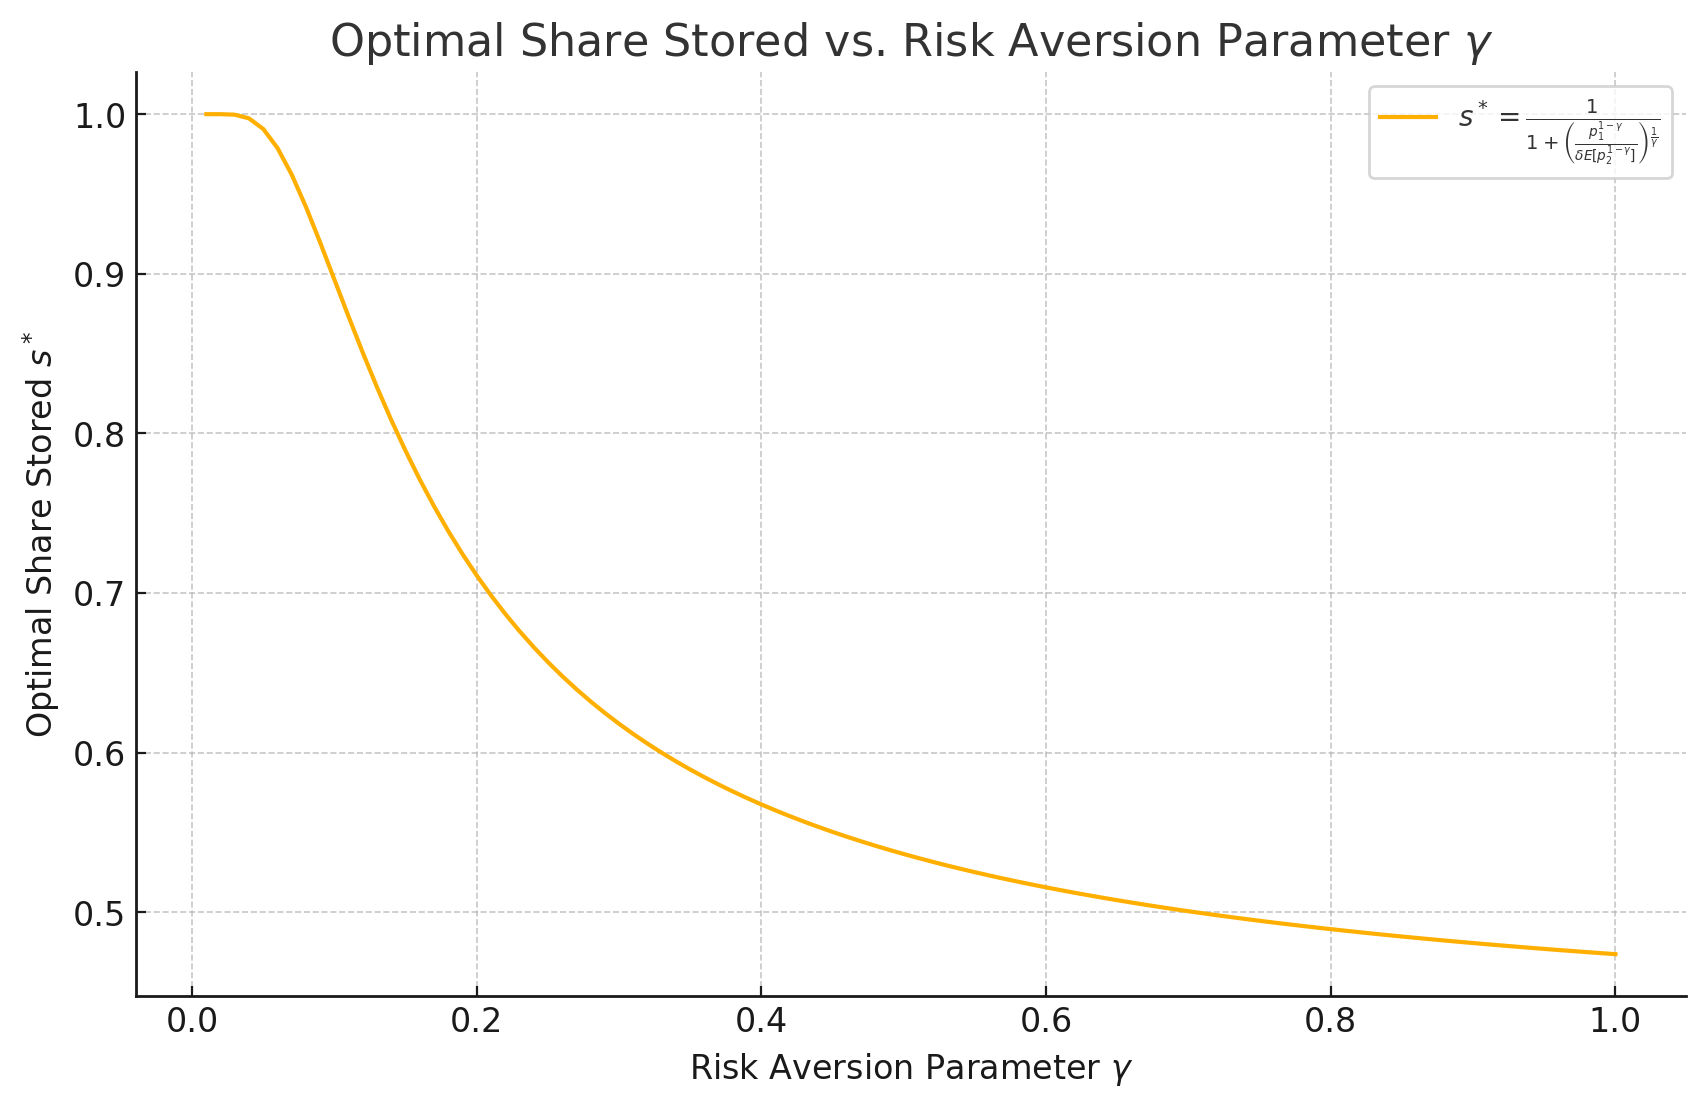
\includegraphics[width=0.45\textwidth]{figures/optimal_s_and_risk_Aversion.png}\label{fig:first}}
    \hfill
    \subfigure[Discount Factor for Different Risk Aversion Levels]{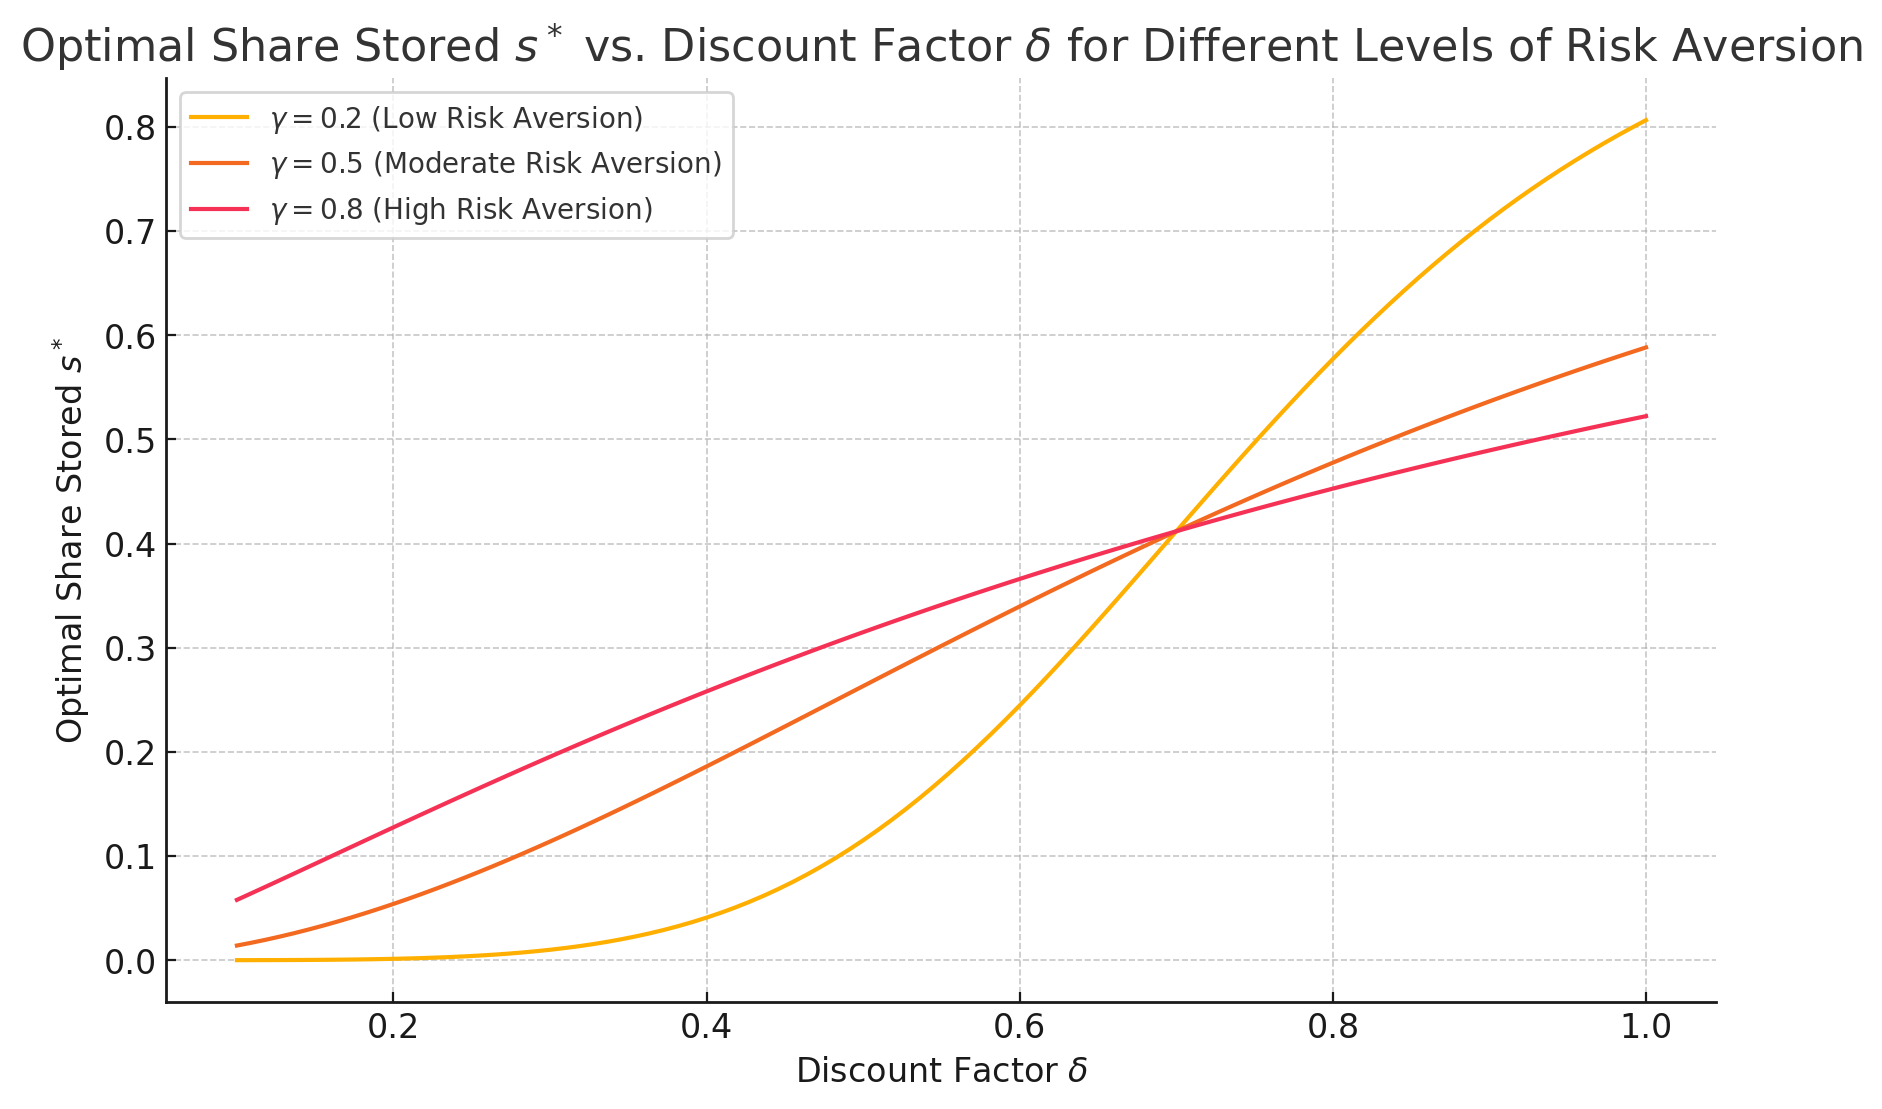
\includegraphics[width=0.45\textwidth]{figures/optimal_s_and_discount_factor.png}\label{fig:second}}
    \caption{The Movement of Optimal $s$}
    \label{fig:model demonstration}
\end{figure}


The left graph below illustrates how the optimal share of the harvest stored (\( s \)) varies with the risk aversion parameter (\( \gamma \)). In this scenario, the first-period price (\( p_1 \)) is held constant at 7, and the expected second-period price (\( E[p_2] \)) is held constant at 10. The horizontal axis represents the risk aversion parameter (\( \gamma \)), while the vertical axis shows the optimal share stored (\( s \)).

As depicted, when the farmer is less risk-averse (lower \( \gamma \)), the optimal storage share tends to be higher. Conversely, as the risk aversion increases (higher \( \gamma \)), the optimal storage share decreases. This relationship highlights that risk-averse farmers prefer to sell more in the first period when they are more concerned about future uncertainties in terms of market competition.


Keeping the prices constant at the same values, the right graph explores the impact of varying the discount factor (\( \delta \)) on the optimal storage decision. This graph features three curves, each representing different levels of risk aversion: low-risk aversion (\( \gamma = 0.2 \) in yellow), moderate risk aversion (\( \gamma = 0.5 \) in orange), and high-risk aversion (\( \gamma = 0.8 \) in red).

As the discount factor increases (storage cost gets lower), the optimal storage share also increases across all levels of risk aversion. This behavior is consistent across all risk aversion levels, though the degree of sensitivity to the discount factor varies. Farmers with lower risk aversion tend to store more as \(\delta\) increases compared to those with moderate and higher risk aversion.


According to \cite{jin2024losses}, whose fieldwork areas are highly overlapped with ours, their risk experiment indicates that the sampled apple growers are generally risk-averse, suggesting a degree of risk aversion close to the CRRA interval [0.437, 0.575). 

\cite{jin2017farmers} obtain information about subjects’ degree of relative risk aversion by assuming that individuals have a constant relative risk aversion utility function, where $r$ is the coefficient of relative risk aversion (CRRA), and $x$ is the payoff in the option. Under this specification, a CRRA coefficient $r > 0$ implies risk aversion, $r = 0$ risk neutrality, and $r < 0$ risk-seeking preferences. Column 5 in Figure \ref{fig:Risk Aversion Experiment Chart} provides the implied CRRA ranges.





% ------------------------------------------ %
% ------------------------------------------ %
% ------------------------------------------ %
\newpage
\section{Traders' Competition: Oligopsonistic Maximization Problem (Cournot)}

To capture the element of time-varying buyer-side competition and incorporate it into the price parameters in the model above, I am considering the Cournot market structure for each trading period from the traders' perspective as follows. 

\subsection{Objective and Profit Function}
In each trading period, each buyer \( i \) aims to maximize their profit \( \pi_i \). The profit for buyer \( i \) is given by:
\begin{equation}
\pi_i = r_i(q_i) - p(Q) q_i
\end{equation}
where:
\begin{itemize}
  \item \( r_i(q_i) \) is the revenue obtained from selling the purchased quantity \( q_i \).
  \item \( p(Q) \) is the inverse supply function representing the price per unit when the total quantity \( Q \) is purchased.
  \item \( q_i \) is the quantity purchased by buyer \( i \).
  \item \( Q \) is the total quantity purchased by all buyers, \( Q = \sum_{j} q_j \).
\end{itemize}

\subsubsection{First-Order Condition (FOC)}
To maximize profit, the buyer will choose \( q_i \) such that the marginal revenue equals the marginal expenditure. The first-order condition (FOC) for maximization is:
\begin{equation}
\frac{\partial \pi_i}{\partial q_i} = \frac{\partial r_i(q_i)}{\partial q_i} - \frac{\partial [p(Q) q_i]}{\partial q_i} = 0
\end{equation}

\subsubsection{Additional Assumptions}
\begin{itemize}
  \item Homogeneous buyers: all buyers are identical.
  \item Perfect Competition in the output market: \( r_i'(q_i) = R \) (marginal revenue is a constant, R, for all buyers). Reasoning behind: Although traders may exercise buyer power in localized procurement markets, they then sell into broader output markets and face competition from traders who operate in different regions.
  \item The derivative of \( Q \) with respect to \( q_i \) is given by:
    \begin{equation}
    \frac{\partial Q}{\partial q_i} = 1 + \lambda
    \end{equation}
  \item The quantity purchased by each buyer is:
    \begin{equation}
    q_i = \frac{Q}{n}
    \end{equation}
    where \( n \) is the number of buyers.
  \item The elasticity of supply is:
    \begin{equation}
    \mu = \frac{\partial Q}{\partial p} \cdot \frac{p}{Q}
    \end{equation}
\end{itemize}

\subsubsection{First-Order Condition again}
\begin{equation}
R = p + \frac{Q}{n} p'(Q) (1 + \lambda)
\end{equation}
Given the elasticity of supply \(\mu\):
\begin{equation}
\mu = \frac{\partial Q}{\partial p} \cdot \frac{p}{Q}
\end{equation}
Inverting to express \(\frac{\partial p}{\partial Q}\):
\begin{equation}
\frac{\partial p}{\partial Q} = \frac{1}{\frac{\partial Q}{\partial p}} = \frac{p}{\mu Q}
\end{equation}
Substitute \( p'(Q) \) into FOC:
\begin{equation}
R = p + \frac{Q}{n} \cdot \frac{p}{\mu Q} \cdot (1 + \lambda)
\end{equation}
Simplifying:
\begin{equation}
R = p + \frac{p}{n \mu} \cdot (1 + \lambda)
\end{equation}
\begin{equation}
R = p \left(1 + \frac{1 + \lambda}{n \mu}\right)
\end{equation}

\subsection{Lerner Index}
\begin{equation}
L = \frac{R - p}{p} = \frac{1 + \lambda}{n \mu}
\end{equation}

\subsection{Optimal Procurement Price}
Starting from:
\begin{equation}
R = p \left(1 + \frac{1 + \lambda}{n \mu}\right)
\end{equation}
Solving for \( p \):
\begin{equation}
p = \frac{R}{1 + \frac{1 + \lambda}{n \mu}}
\end{equation}
Simplify to avoid fraction within a fraction:
\begin{equation}
\textcolor{blue}{p = \frac{R \cdot n \mu}{n \mu + 1 + \lambda}}
\label{Eq: optimal procure price, general case}
\end{equation}



\subsection{Important Notes}
\begin{enumerate}
    \item \textbf{Cartel Solution:} Cartel solution is NOT an NE for any static game, but it may be NE behavior in any single play of an infinite-horizon repeated game. (by Folk Theorem)
    
    \item \textbf{Why Cournot, instead of Bertrand?} Analogy to \cite{kreps1983quantity}, we can infer that when traders simultaneously and independently receive "downstream orders" for subsequent distribution, and we assume that the capacity level (the quantity of the downstream orders) are public information and traders compete in Bertrand-like price competition, with the supply allocated in Bertrand fashion where the provision that one cannot satisfy more supply than one's order from downstream in the first stage: \\
    "Capacity introduced + Bertrand" $\Longleftrightarrow$ "Cournot".

    \item \textbf{Supply Elasticity:} the village supply to this model should be elastic in both periods, but differ in two periods because farmers have the "outside" selling options differently. 
\end{enumerate}


\subsection{Case 1: Linear Supply Function}

\subsubsection*{Problem Setting}

Each buyer \( i \) aims to maximize their profit \( \pi_i \):
\[
\pi_i = r_i(q_i) - (a + bQ)q_i
\]
where \( p = a + bQ \) is the linear supply function.

\subsubsection*{First-Order Condition}

To maximize profit, the first-order condition (FOC) is:
\[
R = \frac{\partial r_i(q_i)}{\partial q_i} = a + bQ + b \frac{Q}{n}
\]
Since \( q_i = \frac{Q}{n} \), the total quantity \( Q \) is:
\[
Q = nq_i
\]
Thus, the FOC simplifies to:
\[
R = a + bQ \left(1 + \frac{1}{n}\right) = a + bQ \left(\frac{n+1}{n}\right)
\]
Rearranging to solve for \( Q \):
\[
R = a + bQ \left(\frac{n+1}{n}\right)
\]
\[
R - a = bQ \left(\frac{n+1}{n}\right)
\]
\[
Q = \frac{n(R - a)}{b(n+1)}
\]

\subsubsection*{Cournot-competition Price}

Substitute \( Q \) back into the supply function:
\[
p = a + bQ
\]
\[
p = a + b \left( \frac{n(R - a)}{b(n+1)} \right)
\]
\[
p = a + \frac{n(R - a)}{n+1}
\]
\begin{equation}
    \textcolor{blue}{p = \frac{a + nR}{n+1}}
    \label{Eq: optimal procure price, linear supply case}
\end{equation}
Thus, the farm-gate price that these middlemen offer to farmers becomes an increasing function of the number of traders showing up ($n$), their marginal value product ($R$), and the farmers' reservation price ($a$).


\section{Challenges Needed to Solve}
Therefore, we may combine the two settings above, by plugging the farm-gate price expressions in either Eq(\ref{Eq: optimal procure price, general case}) or Eq(\ref{Eq: optimal procure price, linear supply case}) back into the optimal share of the harvest to store in Eq(\ref{Eq: KT solution of farmer's max problem}). Therefore, the farmers' storage decisions could depend on their risk aversion, the discount factor (composite storage cost), and the market-structure elements. 


However, there exists a severe issue of inconsistency: in the derivation of the procurement price from the Cournot oligopsonistic setting, I implicitly assume an inverse supply function in each trading period. However, the farmers' maximization problem would actually alter the quantity of local supply hence change the farm-gate price we derive from the traders' perspective. 




\section{Related Literature}
\begin{itemize}
    \item \cite{chiappori2011relative} finds that individuals’ relative risk aversion is indeed constant. 
    
    \item \cite{de2014measuring} use a relatively large lab-in-the-field experiment to explore risk preferences related to sweet potato production among a sample of farmers in northern Mozambique. They reject the null hypothesis that farmers' preferences follow the CRRA utility function, in favor of the more flexible power risk aversion preferences. 

    \item \cite{finger2023stability} find that risk preferences vary considerably over time. Also, they find that farmers' risk preferences change considerably when measured using different methods. For example, self-reported risk preference and findings from a Holt and Laury lottery correlate only weakly. 
    
    \item According to \cite{hardaker2000some}, the relative risk aversion coefficient is a pure number that can be used even in an international comparison of risk aversion.
\end{itemize}

\newpage
\bibliography{reference}


\end{document}
